\documentclass{article}

\usepackage[a4paper]{geometry}
\usepackage[USenglish]{babel}
\usepackage{parskip}

\usepackage{palatino,eulervm}
\linespread{1.25}

\IfFileExists{classico.sty}
  {\usepackage{classico}}
  {\usepackage{biolinum}}

\usepackage{sectsty}
\allsectionsfont{\sffamily}

\usepackage{amsmath}
\usepackage[noend]{algorithm2e}

\usepackage{tikz}
\usetikzlibrary{positioning}

% NOTE: to compile, place `tikz-uml.sty` in the same folder
\usepackage{tikz-uml}

\let\Star\star
\renewcommand{\star}{$\Star$~}

\begin{document}
\pagestyle{empty}
\newgeometry{top=1cm,bottom=1cm,left=1cm,right=1cm}
\star denotes synthesized attributes (getters)

\begin{center}
\begin{tikzpicture}
% Model
\umlclass{Model}{
+ name: string \\
+ initialState: State \\
\star actions: map of string to Action \\
\star labels: map of string to StateLabel
}{
+ nextStates(s: State): iter of tuple of (State, Action) \\
+ enabled(s: State): set of Action \\
+ stubborn(s: State): set of Action \\
+ reach(): iter of State
}

% State
\umlclass[below left=0.5cm of Model]{State}{
\star labels: set of StateLabel
}{
+ clone(): State
}
\umluniassoc[geometry=-|,arg1=model,mult1=1,mult2=*]{State}{Model}

% SlotState
\umlclass[below=1cm of State]{SlotState}{
+ names: list of string \\
+ slots: any \\
}{
+ clone(): State
}
\umlimpl{SlotState}{State}

% Action
\umlclass[below right=0.5cm of Model]{Action}{
+ id: string \\
+ guards: set of StateLabel \\
+/\star DNA: set of Action \\[1em]
+ commute: set of Action \\[1em]
+ reads: set of string \\
+ writes: set of string \\
\star tests: set of string \\
\star vars: set of string \\[1em]
\star score: integer \\
}{
+ accords(a: Action): bool
}
\umluniassoc[geometry=-|,arg1=model,mult1=1,mult2=*]{Action}{Model}

% StateLabel
\umlclass[below=0.5cm of Action]{StateLabel}{
+ id: string \\
+/\star NES: set of Action \\
+ NDS: set of Action \\
+ coenable: set of StateLabel \\
+ tests: set of string \\[1em]
+ cost: integer \\
}{
}
\umluniassoc[geometry=-|,arg1=model,mult1=1,mult2=*]{StateLabel}{Model}
\end{tikzpicture}
\end{center}

\end{document}
